\documentclass{ucll-slides}
\usepackage{pxfonts}
\usepackage{tikz}
\usepackage{calc}
\usepackage{ucll-code}


\usetikzlibrary{calc,shadows,tikzmark}

\coursename{Elixir Learning Materials}
\title{linked lists and arrays}



\pgfkeys{
  /custom/.cd,
  width/.initial=1cm,
  height/.initial=1cm,
  position/.initial={0,0},
  size/.style={width=#1,height=#1},
  value/.initial={},
  value font/.initial={\ttfamily}
}

\newcommand{\llnode}[1][1]{
    {
        \pgfkeys{/custom/.cd,#1}
        \pgfkeys{/custom/width/.get=\llnodewidth}
        \pgfkeys{/custom/height/.get=\llnodeheight}
        \pgfkeys{/custom/position/.get=\llnodeposition}
        \pgfkeys{/custom/value/.get=\llnodevalue}
        \pgfkeys{/custom/value font/.get=\llnodevaluefont}
        \draw[thick] (\llnodeposition) rectangle ++(\llnodewidth,\llnodeheight);
        \draw[thick] ($ (\llnodeposition) + (\llnodewidth,0) $) rectangle ++(\llnodewidth,\llnodeheight);
        \node[font=\llnodevaluefont] at ($ (\llnodeposition) + (\llnodewidth / 2,\llnodeheight / 2) $) {\llnodevalue};
    }
}

\begin{document}

\maketitle

\begin{frame}
    \frametitle{General information}
    \begin{center}
        \begin{itemize}
            \item Brecht Philtjens
            \item Wannes Fransen
        \end{itemize}
    \end{center}
    \footnotetext{License: Creative Commons Attribution-NonCommercial-ShareAlike 4.0 International (CC BY-NC-SA 4.0)}
\end{frame}
\begin{frame}
    \frametitle{Overview}
    \begin{itemize}
        \item Comparison between
              \begin{itemize}
                  \item Arrays
                  \item Linked lists
              \end{itemize}
              \vskip4mm
        \item Purely functional implementation
              \begin{itemize}
                \item Modifications are forbidden
                \item Only creation of new objects is allowed
              \end{itemize}
    \end{itemize}
\end{frame}

\section{Memory Layout}

\frame{\tableofcontents[currentsection]}

\begin{frame}
    \frametitle{Arrays}
    \begin{center}
        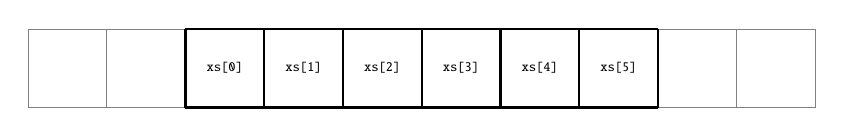
\begin{tikzpicture}
            \draw[help lines] (-2,0) grid (8,1);
            \draw[thick] (0,0) grid (6,1);
            \foreach \x in {0,...,5} {
                \node[font=\tiny] at ($ (\x,0.5) + (0.5,0) $) { \texttt{xs[\x]} };
            }
        \end{tikzpicture}
    \end{center}
    \vskip4mm
    \begin{itemize}
        \item One piece of contiguous memory
    \end{itemize}
\end{frame}

\begin{frame}
    \frametitle{Arrays}
    \code[language=c++14]{array.cpp}
\end{frame}

\begin{frame}
    \frametitle{Linked Lists}
    \begin{center}
        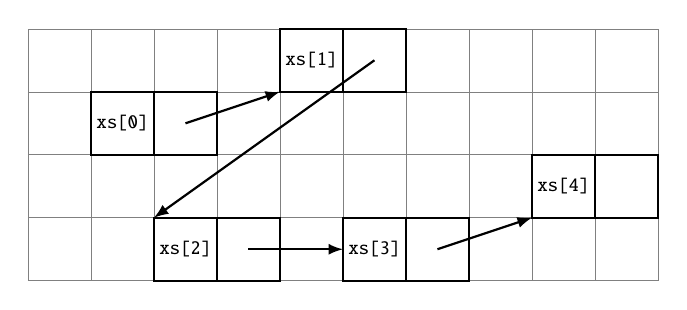
\begin{tikzpicture}[link/.style={thick,-latex},scale=0.8,transform shape]
            \coordinate (p1) at (1,2);
            \coordinate (p2) at (4,3);
            \coordinate (p3) at (2,0);
            \coordinate (p4) at (5,0);
            \coordinate (p5) at (8,1);

            \draw[help lines] (0,0) grid (10,4);
            \foreach[evaluate={int(\i-1)} as \j] \i in {1,...,5} {
                \llnode[position={p\i},value={xs[\j]},value font=\ttfamily\small]
            }

            \draw[link] ($ (p1) + (1.5, 0.5) $) -- ($ (p2) $);
            \draw[link] ($ (p2) + (1.5, 0.5) $) -- ($ (p3) + (0,1) $);
            \draw[link] ($ (p3) + (1.5, 0.5) $) -- ($ (p4) + (0,0.5) $);
            \draw[link] ($ (p4) + (1.5, 0.5) $) -- ($ (p5) $);
        \end{tikzpicture}
    \end{center}
    \vskip4mm
    \begin{itemize}
        \item List consists of series of nodes
        \item Each node has two fields
              \begin{itemize}
                \item Item
                \item Reference to next node
              \end{itemize}
        \item Nodes scattered across memory
    \end{itemize}
\end{frame}

\begin{frame}
    \frametitle{Linked Lists in Code}
    \code[language=csharp]{LinkedList.cs}
\end{frame}

\begin{frame}
    \frametitle{Creating a Linked List}
    \begin{center}
        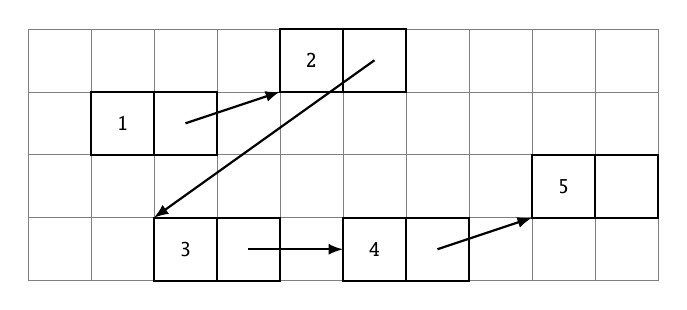
\begin{tikzpicture}[link/.style={thick,-latex},scale=0.8,transform shape]
            \coordinate (p1) at (1,2);
            \coordinate (p2) at (4,3);
            \coordinate (p3) at (2,0);
            \coordinate (p4) at (5,0);
            \coordinate (p5) at (8,1);

            \draw[help lines] (0,0) grid (10,4);
            \foreach \i in {1,...,5} {
                \llnode[position=p\i,value=\i]
            }

            \draw[link] ($ (p1) + (1.5, 0.5) $) -- ($ (p2) $);
            \draw[link] ($ (p2) + (1.5, 0.5) $) -- ($ (p3) + (0,1) $);
            \draw[link] ($ (p3) + (1.5, 0.5) $) -- ($ (p4) + (0,0.5) $);
            \draw[link] ($ (p4) + (1.5, 0.5) $) -- ($ (p5) $);
        \end{tikzpicture}
    \end{center}
    \vskip4mm
    \code[language=csharp]{LinkedListCreation.cs}
\end{frame}
\section{Determining Length}

\frame{\tableofcontents[currentsection]}

\begin{frame}
    \frametitle{Problem Statement}
    \begin{center}\ttfamily
        len([1,2,3,4,5,6,7]) \\[4mm]
        $\downarrow$ \\[4mm]
        7
    \end{center}
\end{frame}

\begin{frame}
    \frametitle{Length of Array}
    \begin{itemize}
        \item Array must keep track of  length
        \item Computing length is immediate
        \item $O(1)$
    \end{itemize}
\end{frame}

\begin{frame}
    \frametitle{Length of Linked List}
    \begin{center}
        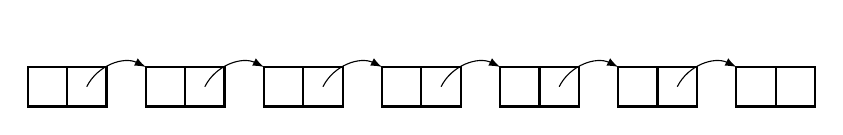
\begin{tikzpicture}[link/.style={thick,-latex}]
            \path[use as bounding box] (0,0) rectangle (10,1);

            \foreach[count=\i] \x in {0,1.5,...,10} {
                \coordinate (p\i) at (\x,0);
                \llnode[position={p\i},size=0.5cm]
            }

            \foreach[count=\i] \x in {0,1.5,...,8} {
                \draw[-latex] ($ (p\i) + (0.75,0.25) $) to[bend left=45] ++(0.75,0.251);
            }
        \end{tikzpicture}
    \end{center}
    \vskip4mm
    \structure{Algorithm}
    \begin{itemize}
        \item Follow nodes until we find \texttt{null}
        \item Count number of jumps necessary
        \item Takes longer for longer lists
        \item $O(n)$
    \end{itemize}
\end{frame}
\section{Indexing}

\frame{\tableofcontents[currentsection]}

\begin{frame}
    \frametitle{Problem Statement}
    \begin{center}\ttfamily
        [1, 2, 3, 4, 5, 6][3] \\[4mm]
        $\downarrow$ \\[4mm]
        4
    \end{center}
\end{frame}

\begin{frame}
    \frametitle{Indexing Array}
    \begin{center}
        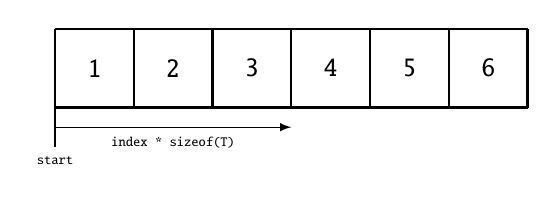
\begin{tikzpicture}
            \draw[thick] (0,0) grid (6,1);
            \foreach[evaluate={int(\x+1)} as \i] \x in {0,...,5} {
                \node[font=\ttfamily] at ($ (\x,0.5) + (0.5,0) $) {\i};
            }
            \draw[thick] (0,0) -- ++(0,-0.5);
            \node[anchor=north,font=\ttfamily\tiny] at (0,-0.5) {start};
            \draw[|-latex] (0,-.25) -- ++(3,0) node[midway,below,font=\tiny\ttfamily] {index * sizeof(T)};
        \end{tikzpicture}
    \end{center}
    \vskip4mm
    \structure{Algorithm}
    \begin{itemize}
        \item Memory location can be computed in a single step
        \item \texttt{location = start + index * sizeof(T)}
        \item Direct CPU support: only 1 instruction required
        \item Explains zero-indexing
        \item $O(1)$
    \end{itemize}
\end{frame}

\begin{frame}
    \frametitle{Indexing Linked List}
    \begin{center}
        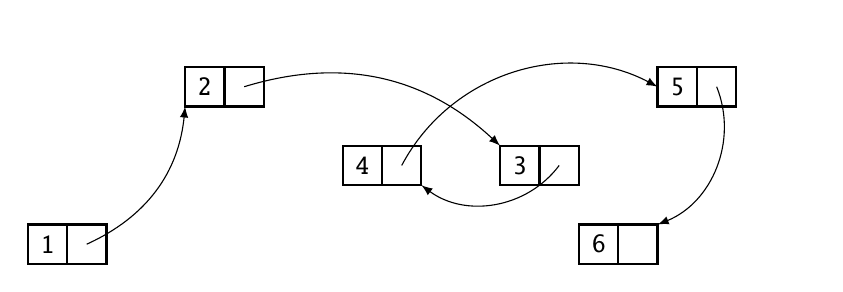
\begin{tikzpicture}[link/.style={thick,-latex}]
            \path[use as bounding box] (0,0) rectangle (10,3);
            \coordinate (p1) at (0,0);
            \coordinate (p2) at (2,2);
            \coordinate (p4) at (4,1);
            \coordinate (p3) at (6,1);
            \coordinate (p5) at (8,2);
            \coordinate (p6) at (7,0);

            \foreach \i in {1,...,6} {
                \llnode[position={p\i},size=0.5cm,value=\i]
            }

            \draw[-latex] ($ (p1) + (0.75,0.25) $) to[bend right=30] (p2);
            \draw[-latex] ($ (p2) + (0.75,0.25) $) to[bend left=30] ($ (p3) + (0,0.5) $);
            \draw[-latex] ($ (p3) + (0.75,0.25) $) to[bend left=45] ($ (p4) + (1,0) $);
            \draw[-latex] ($ (p4) + (0.75,0.25) $) to[bend left=45] ($ (p5) + (0,0.25) $);
            \draw[-latex] ($ (p5) + (0.75,0.25) $) to[bend left=45] ($ (p6) + (1,0.5) $);
        \end{tikzpicture}
    \end{center}
    \vskip4mm
    \structure{Algorithm}
    \begin{itemize}
        \item Nodes are scattered unpredictably across memory
        \item Follow \texttt{Next} until \texttt{Next == null}
        \item Finding \texttt{n}th element takes \texttt{n} jumps
        \item $O(n)$
    \end{itemize}
\end{frame}

\section{Updating}

\frame{\tableofcontents[currentsection]}

\begin{frame}
    \frametitle{Problem Statement}
    \begin{center} \ttfamily
         [1, 2, 3, 4, 5, 6][3] = 0
         $\downarrow$ \\[4mm]
         [1, 2, 3, 0, 5, 6]
    \end{center}
\end{frame}

\begin{frame}
    \frametitle{Updating an Array}
    \begin{center}
        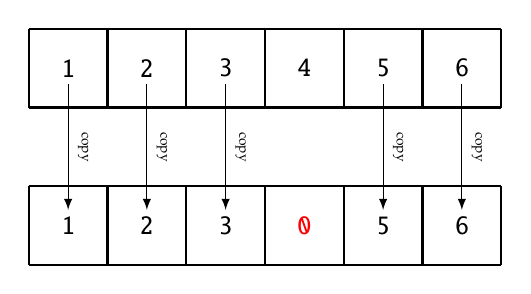
\begin{tikzpicture}
            \draw[thick] (0,0) grid ++(6,1);
            \foreach[evaluate={int(\i+1)} as \j] \i in {0,...,5} {
                \node[font=\ttfamily] at (\i + 0.5,0.5) {\j};
            }
            \foreach[evaluate={int(\i+1)} as \j] \i in {0,1,2,4,5} {
                \node[font=\ttfamily] at (\i + 0.5,-1.5) {\j};
            }
            \node[red,font=\ttfamily] at (3.5,-1.5) {0};

            \draw[thick] (0,-2) grid ++(6,1);

            \foreach \i in {0,1,2,4,5} {
                \draw[-latex] (\i + 0.5,0.3) -- (\i + 0.5,-1.3) node[midway,sloped,font=\tiny,above] {copy};
            }
        \end{tikzpicture}
    \end{center}
    \vskip4mm
    \structure{Algorithm}
    \begin{itemize}
        \item Requires copying entire array
        \item $O(n)$
    \end{itemize}
\end{frame}

\begin{frame}
    \frametitle{Updating a Linked List}
    \begin{center}
        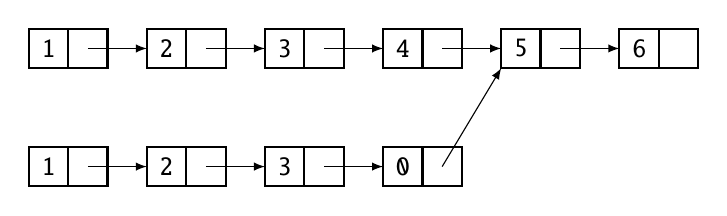
\begin{tikzpicture}[link/.style={thick,-latex}]
            \foreach[evaluate={(\i-1) * 1.5} as \x] \i in {1,...,6} {
                \coordinate (p\i) at (\x,0);
                \llnode[position={p\i},size=0.5cm,value=\i]
            }

            \foreach[evaluate={(\i-1) * 1.5} as \x] \i/\v in {1/1,2/2,3/3,4/0} {
                \coordinate (q\i) at (\x,-1.5);
                \llnode[position={q\i},size=0.5cm,value=\v]
            }

            \foreach[evaluate={(\i-1) * 1.5} as \x] \i in {1,...,5} {
                \draw[-latex] ($ (p\i) + (0.75,0.25) $) -- ++(0.75,0);
            }

            \foreach[evaluate={(\i-1) * 1.5} as \x] \i in {1,2,3} {
                \draw[-latex] ($ (q\i) + (0.75,0.25) $) -- ++(0.75,0);
            }

            \draw[-latex] ($ (q4) + (0.75,0.25) $) -- ($ (p5) $);
        \end{tikzpicture}
    \end{center}
    \vskip4mm
    \structure{Algorithm}
    \begin{itemize}
        \item Create new list
        \item Nodes after modified element can be reused
        \item $O(n)$
    \end{itemize}
\end{frame}

\section{Adding to Front}

\frame{\tableofcontents[currentsection]}

\begin{frame}
    \frametitle{Problem Statement}
    \begin{center}\ttfamily
        prepend([1, 2, 3, 4, 5], 0) \\[4mm]
        $\downarrow$ \\[4mm]
        [0, 1, 2, 3, 4, 5]
    \end{center}
\end{frame}

\begin{frame}
    \frametitle{Add to Front of Array}
    \begin{center}
        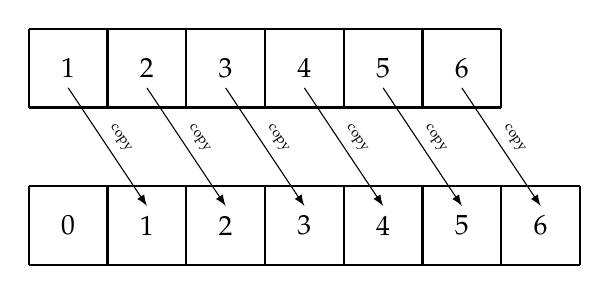
\begin{tikzpicture}
            \draw[thick] (0,0) grid ++(6,1);
            \draw[thick] (0,-2) grid ++(7,1);

            \foreach[evaluate={int(\i+1)} as \j] \i in {0,...,5} {
                \node at (\i + 0.5,0.5) {\j};
                \node at (\i + 1.5,-1.5) {\j};
                \draw[-latex] (\i + 0.5,0.25) -- (\i + 1.5,-1.25) node[midway,sloped,font=\tiny,above] {copy};
            }

            \node at (0.5,-1.5) {0};
        \end{tikzpicture}
    \end{center}
    \vskip4mm
    \structure{Algorithm}
    \begin{itemize}
        \item Create new array with larger size
        \item Copy all elements
        \item $O(n)$
    \end{itemize}
\end{frame}

\begin{frame}
    \frametitle{Add to Front of Linked List}
    \begin{center}
        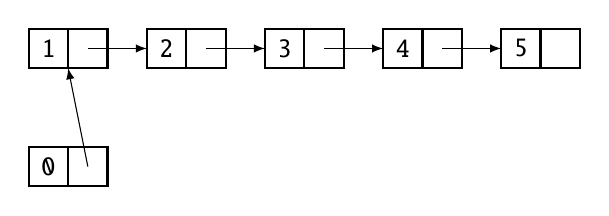
\begin{tikzpicture}[link/.style={thick,-latex}]
            \foreach[evaluate={(\i - 1) * 1.5} as \x] \i in {1,...,5} {
                \coordinate (p\i) at (\x,0);
                \llnode[position={p\i},size=0.5cm,value=\i]
            }

            \foreach[evaluate={(\i - 1) * 1.5} as \x] \i in {1,...,4} {
                \draw[-latex] ($ (p\i) + (0.75,0.25) $) -- ++(0.75,0);
            }

            \coordinate (p0) at ($ (p1) + (0,-1.5) $);
            \llnode[position=p0,size=0.5cm,value=0]
            \draw[-latex] ($ (p0) + (0.75,0.25) $) -- ($ (p1) + (0.5,0) $);
        \end{tikzpicture}
    \end{center}
    \vskip4mm
    \structure{Algorithm}
    \begin{itemize}
        \item Create new node
        \item Have it point to the (originally) first node
        \item $O(1)$
    \end{itemize}
\end{frame}

\section{Concatenation}

\frame{\tableofcontents[currentsection]}

\begin{frame}
    \frametitle{Problem Statement}
    \begin{center} \ttfamily
         [1,2,3,4,5] ++ [6,7,8,9,10,11,12,13]\\[4mm]
         $\downarrow$ \\[4mm]
         [1,2,3,4,5,6,7,8,9,10,11,12,13]
    \end{center}
\end{frame}

\begin{frame}
    \frametitle{Updating an Array}
    \begin{center}
        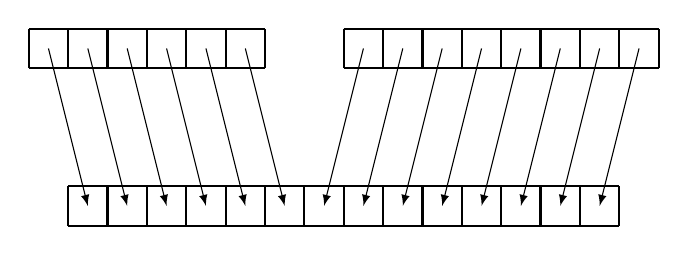
\begin{tikzpicture}
            \draw[thick] (0,0) grid[step=0.5cm] ++(3,0.5);
            \draw[thick,xshift=4cm] (0,0) grid[step=0.5cm] ++(4,0.5);
            \draw[thick,xshift=0.5cm] (0,-2) grid[step=0.5cm] ++(7,0.5);

            \foreach \i in {0,0.5,...,2.5} {
                \draw[-latex] (\i+0.25,0.25) -- (\i+0.75,-1.75);
            }

            \foreach \i in {0,0.5,...,3.5} {
                \draw[-latex] (\i+4.25,0.25) -- (\i+3.75,-1.75);
            }
        \end{tikzpicture}
    \end{center}
    \vskip4mm
    \structure{Algorithm}
    \begin{itemize}
        \item Requires both arries to be copied
        \item $O(n_1 + n_2)$
    \end{itemize}
\end{frame}

\begin{frame}
    \frametitle{Updating a Linked List}
    \begin{center}
        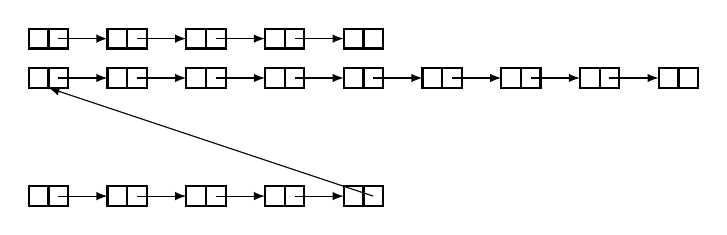
\begin{tikzpicture}[link/.style={thick,-latex}]
            \foreach[count=\i] \x in {0,...,4} {
                \coordinate (p\i) at (\x,0);
                \llnode[position=p\i,size=0.25cm]
            }

            \foreach[evaluate={\i+1} as \j] \i in {1,...,4} {
                \draw[-latex] ($ (p\i) + (0.375,0.125) $) -- ($ (p\j) + (0,0.125) $);
            }

            \foreach[count=\i] \x in {0,...,8} {
                \coordinate (q\i) at (\x,-0.5);
                \llnode[position=q\i,size=0.25cm]
            }

            \foreach[evaluate={\i+1} as \j] \i in {1,...,8} {
                \draw[-latex] ($ (q\i) + (0.375,0.125) $) -- ($ (q\j) + (0,0.125) $);
            }

            \foreach[count=\i] \x in {0,...,4} {
                \coordinate (r\i) at (\x,-2);
                \llnode[position=r\i,size=0.25cm]
            }

            \foreach[evaluate={\i+1} as \j] \i in {1,...,4} {
                \draw[-latex] ($ (r\i) + (0.375,0.125) $) -- ($ (r\j) + (0,0.125) $);
            }
            \draw[-latex] ($ (r5) + (0.375,0.125) $) -- ($ (q1) + (0.25,0) $);
        \end{tikzpicture}
    \end{center}
    \vskip4mm
    \structure{Algorithm}
    \begin{itemize}
        \item Only first list needs to be copied
        \item Second list can be safely reused
        \item Copy's last node points to second list's first node
        \item $O(n_1)$
    \end{itemize}
\end{frame}

\section{Conclusion}

\frame{\tableofcontents[currentsection]}

\begin{frame}
    \frametitle{Comparison}
    \begin{center}
        \begin{tabular}{lcc}
            & \textbf{Array} & \textbf{Linked List} \\
            \midrule
            Length & $O(1)$ & $O(n)$ \\
            Indexing & $O(1)$ & $O(n)$ \\
            Updating & $O(n)$ & $O(n)$ \\
            Add to front & $O(n)$ & $O(1)$ \\
            Concatenation & $O(n_1+n_2)$ & $O(n_1)$ \\
            \bottomrule
        \end{tabular}
    \end{center}
\end{frame}

\begin{frame}
    \frametitle{Usage}
    \begin{itemize}
        \item Linked lists are often used for sequential processing
              \begin{itemize}
                \item Move left to right
                \item No indexing necessary
                \item Build new list as you go
              \end{itemize}
        \item Don't treat linked lists as if they were arrays!
    \end{itemize}
\end{frame}

\end{document}

%%% Local Variables:
%%% mode: latex
%%% TeX-master: t
%%% End:
